\documentclass[handout]{ximera}

\title{A new Ximera Activity}
\author{Kelly Stady}

\begin{document}
\begin{abstract}
    Trying this out!
\end{abstract}
\maketitle


\begin{question}
    $2+3=\answer{5}$

\begin{hint}
Think about how many fingers you have on one hand.
\end{hint}

\end{question}




\begin{center} %% Image is found in xmPictures
\textbf{Maple Grpah} \\

    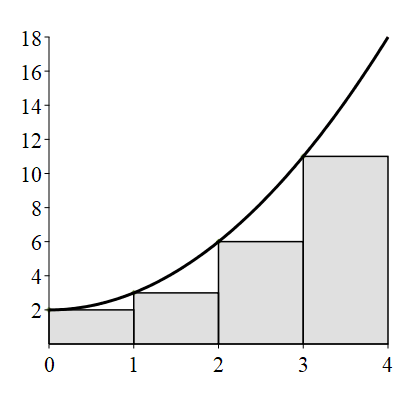
\includegraphics{reimannlo.png}
\end{center}


\begin{question}
 The circle below has been divided into 10 equal parts.  What fraction of the circle is shaded? \\ \\


\begin{center} 
\hspace{0.8in} \begin{tikzpicture}
\draw[thick] (0,0) circle [radius=1.3cm];
\foreach \i in {36,72,...,360}
  \draw[semithick] (0,0)--(\i:1.3cm);    %The colon signifies that polar coordinates are being used. (60:.75cm) means the point that is at an angle of 60° and a distance of 0.75cm from the origin. Length of radial lines - should match radius above.
   \draw[thick, fill=glaucous!60] (0,0) --  (36:1.3) arc(36:0:1.3); %To Draw Arc: \draw (x,y) arc (start:stop:radius);
   \draw[thick, fill=glaucous!60] (0,0) --  (72:1.3) arc(72:36:1.3); %Colon indicates polar coordintes (angle:length)
   \draw[thick, fill=glaucous!60] (0,0) --  (108:1.3) arc(108:72:1.3);
 %\draw[fill=glaucous] (0,0) -- (360:1.5) arc(360:324:1.5);

\end{tikzpicture}
\end{center}

\begin{multipleChoice}
\choice[correct]{$\displaystyle \frac{3}{10}$}
\choice{$\displaystyle \frac{1}{10}$}
\choice{$\displaystyle \frac{7}{10}$}
\end{multipleChoice}

\end{question}

\begin{definition}[\textbf{Pythagorean Theorem}]
    $a^2+b^2 = c^2$
\end{definition}    


\begin{exercise}
Evaluate the limit.

\[ \lim\limits_{x \to 2} x^2 = \answer{4} \]

\end{exercise}


\begin{question} Use a limit, with proper notation, to describe the behavior of the function $f(x)=\ln x$ as $x$ approaches $1.$  \textbf{Select all that apply}. \\ \\

    \begin{center} 
        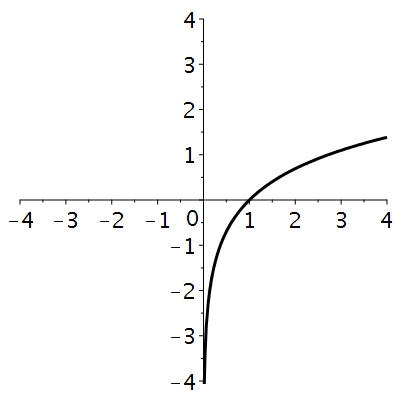
\includegraphics[height=3in, width=3in]{lnplot.png}
    \end{center}

\begin{selectAll}
    \choice[correct]{$\displaystyle \lim\limits_{x \to 1} f(x) = 0$}
    \choice{$\displaystyle \lim\limits_{x \to 1} x = \ln 1$}
    \choice{$\displaystyle \lim\limits_{x \to 1} = 0$}
    \choice[correct]{$\displaystyle \lim\limits_{x \to 1} \ln x = 0$}
    \choice{$\displaystyle \lim f(x)= 0$}
    \choice{$\displaystyle \lim\limits_{x \to 1} f(x) = 1$}
    \choice{$\displaystyle \lim\limits_{x \to 1} \ln x = 1$}
    \end{selectAll}
    \end{question}

\begin{theorem}

\textbf{Addition Property of Equality} \\ 

If $ a = b,$ then $a + c = b + c$.
\end{theorem}


\end{document}
